\newpage
\chapter{Metodologia}
\label{chap:metodologia}

A metodologia desenvolvida consiste em um sistema dual de processamento de dados e classificação adaptativa não supervisionada para detecção de estados operacionais de equipamentos industriais. O sistema foi projetado para operar com dados reais de sensores IoT de diferentes tipos de equipamentos, tratando desafios práticos como lacunas temporais, \textit{outliers}, sincronização de múltiplas fontes e adaptação automática ao tipo de equipamento.

O processo metodológico inicia com a detecção automática do tipo de equipamento baseada nos arquivos de dados disponíveis e em verificações robustas de densidade de cobertura. Originalmente, o sistema exigia que pelo menos 30\% dos dados de corrente e RPM fossem válidos (não nulos) para prosseguir com a classificação elétrica. Entretanto, verificou-se que esta regra estatística relativa penalizava injustamente equipamentos que operam esporadicamente e passam a maior parte do tempo desligados (quando o sensor não gera estimativas elétricas). Para solucionar este viés, a lógica foi refinada para adotar um limite absoluto: se o arquivo \texttt{estimated} possuir pelo menos 1.000 registros reais e válidos de corrente ou RPM (mesmo que representem uma fração percentual mínima de um longo histórico), o equipamento é mantido e processado pelo \textit{pipeline} elétrico. Essa mesma verificação absoluta é imposta estritamente dentro da fase de clusterização e avaliação física do K-Means, garantindo que o algoritmo não descarte variáveis como corrente ou RPM sob a falsa premissa de insuficiência de dados relativos. Equipamentos elétricos ideais possuem este arquivo além de \texttt{validated\_default} e \texttt{validated\_slip}, enquanto equipamentos mecânicos possuem apenas os dois últimos.

Entretanto, em cenários industriais reais, a inferência de dados elétricos como corrente e RPM a partir de sensores IoT baseia-se na análise espectral do fluxo magnético parasita e depende fundamentalmente da configuração da quantidade de polos do motor e de parâmetros de placa exatos na base relacional~\cite{romary2022airgap, doe2014motor, garcia2025estimation}. Quando esses dados cadastrais estão ausentes ou incorretos, o equipamento, mesmo possuindo sensores magnéticos e magnetômetro físicos, não consegue realizar o cálculo de inferência, resultando em valores nulos (\textit{NaN}) para corrente e RPM. Nestes casos específicos, o sistema aplica um \textit{fallback} automático de redundância: o equipamento elétrico é reclassificado e tratado como mecânico. Esta abordagem demonstrou-se altamente eficaz, uma vez que o modelo K-Means utilizando as 16 \textit{features} mecânicas (focadas em temperatura, vibração global/espectral e magnetômetro bruto) consegue distinguir os estados operacionais perfeitamente sem depender das estimativas elétricas falhas. Esta detecção automática permite selecionar o \textit{pipeline} correto, adaptar a estratégia de classificação e configurar visualizações apropriadas.

\section{Visão Geral dos \textit{Pipelines}}

O sistema implementa dois \textit{pipelines} especializados com etapas compartilhadas e específicas. O \textit{pipeline} elétrico processa equipamentos com corrente e RPM através de coleta de dados (\texttt{validated\_default}, \texttt{estimated} e \texttt{validated\_slip}), segmentação e validação de períodos contínuos, processamento e interpolação com KNN temporal e Spline Hermitiana, além do tratamento de \textit{outliers}, junção e sincronização de múltiplas fontes com diferentes frequências, normalização MinMax com \textit{clipping} de \textit{outliers} (percentil 99,5\%), e classificação K-Means com \textit{score} baseado em corrente (peso 2,0), RPM (peso 2,0), vibração (peso 1,0) e temperatura (peso 0,5).

O \textit{pipeline} mecânico processa equipamentos sem inferência de corrente e RPM pelo sensor de campo eletromagnético, através de coleta de dados (\texttt{validated\_default} e \texttt{validated\_slip}), seguindo as mesmas etapas de segmentação, processamento, junção e normalização, mas com classificação K-Means adaptada com \textit{score} baseado em temperatura (peso 1,5), vibração (peso 1,0) e magnetômetro (peso 0,5). Cada etapa é implementada como um \textit{script} Python independente, permitindo modularidade, fácil manutenção e adaptação para novos tipos de equipamentos.

A Figura~\ref{fig:pipeline_treino} apresenta o fluxo completo da etapa de treinamento para a construção dos modelos, abrangendo desde a configuração inicial de \textit{features} até a geração final de modelos e \textit{thresholds} físicos.

\begin{figure}[H]
    \centering
    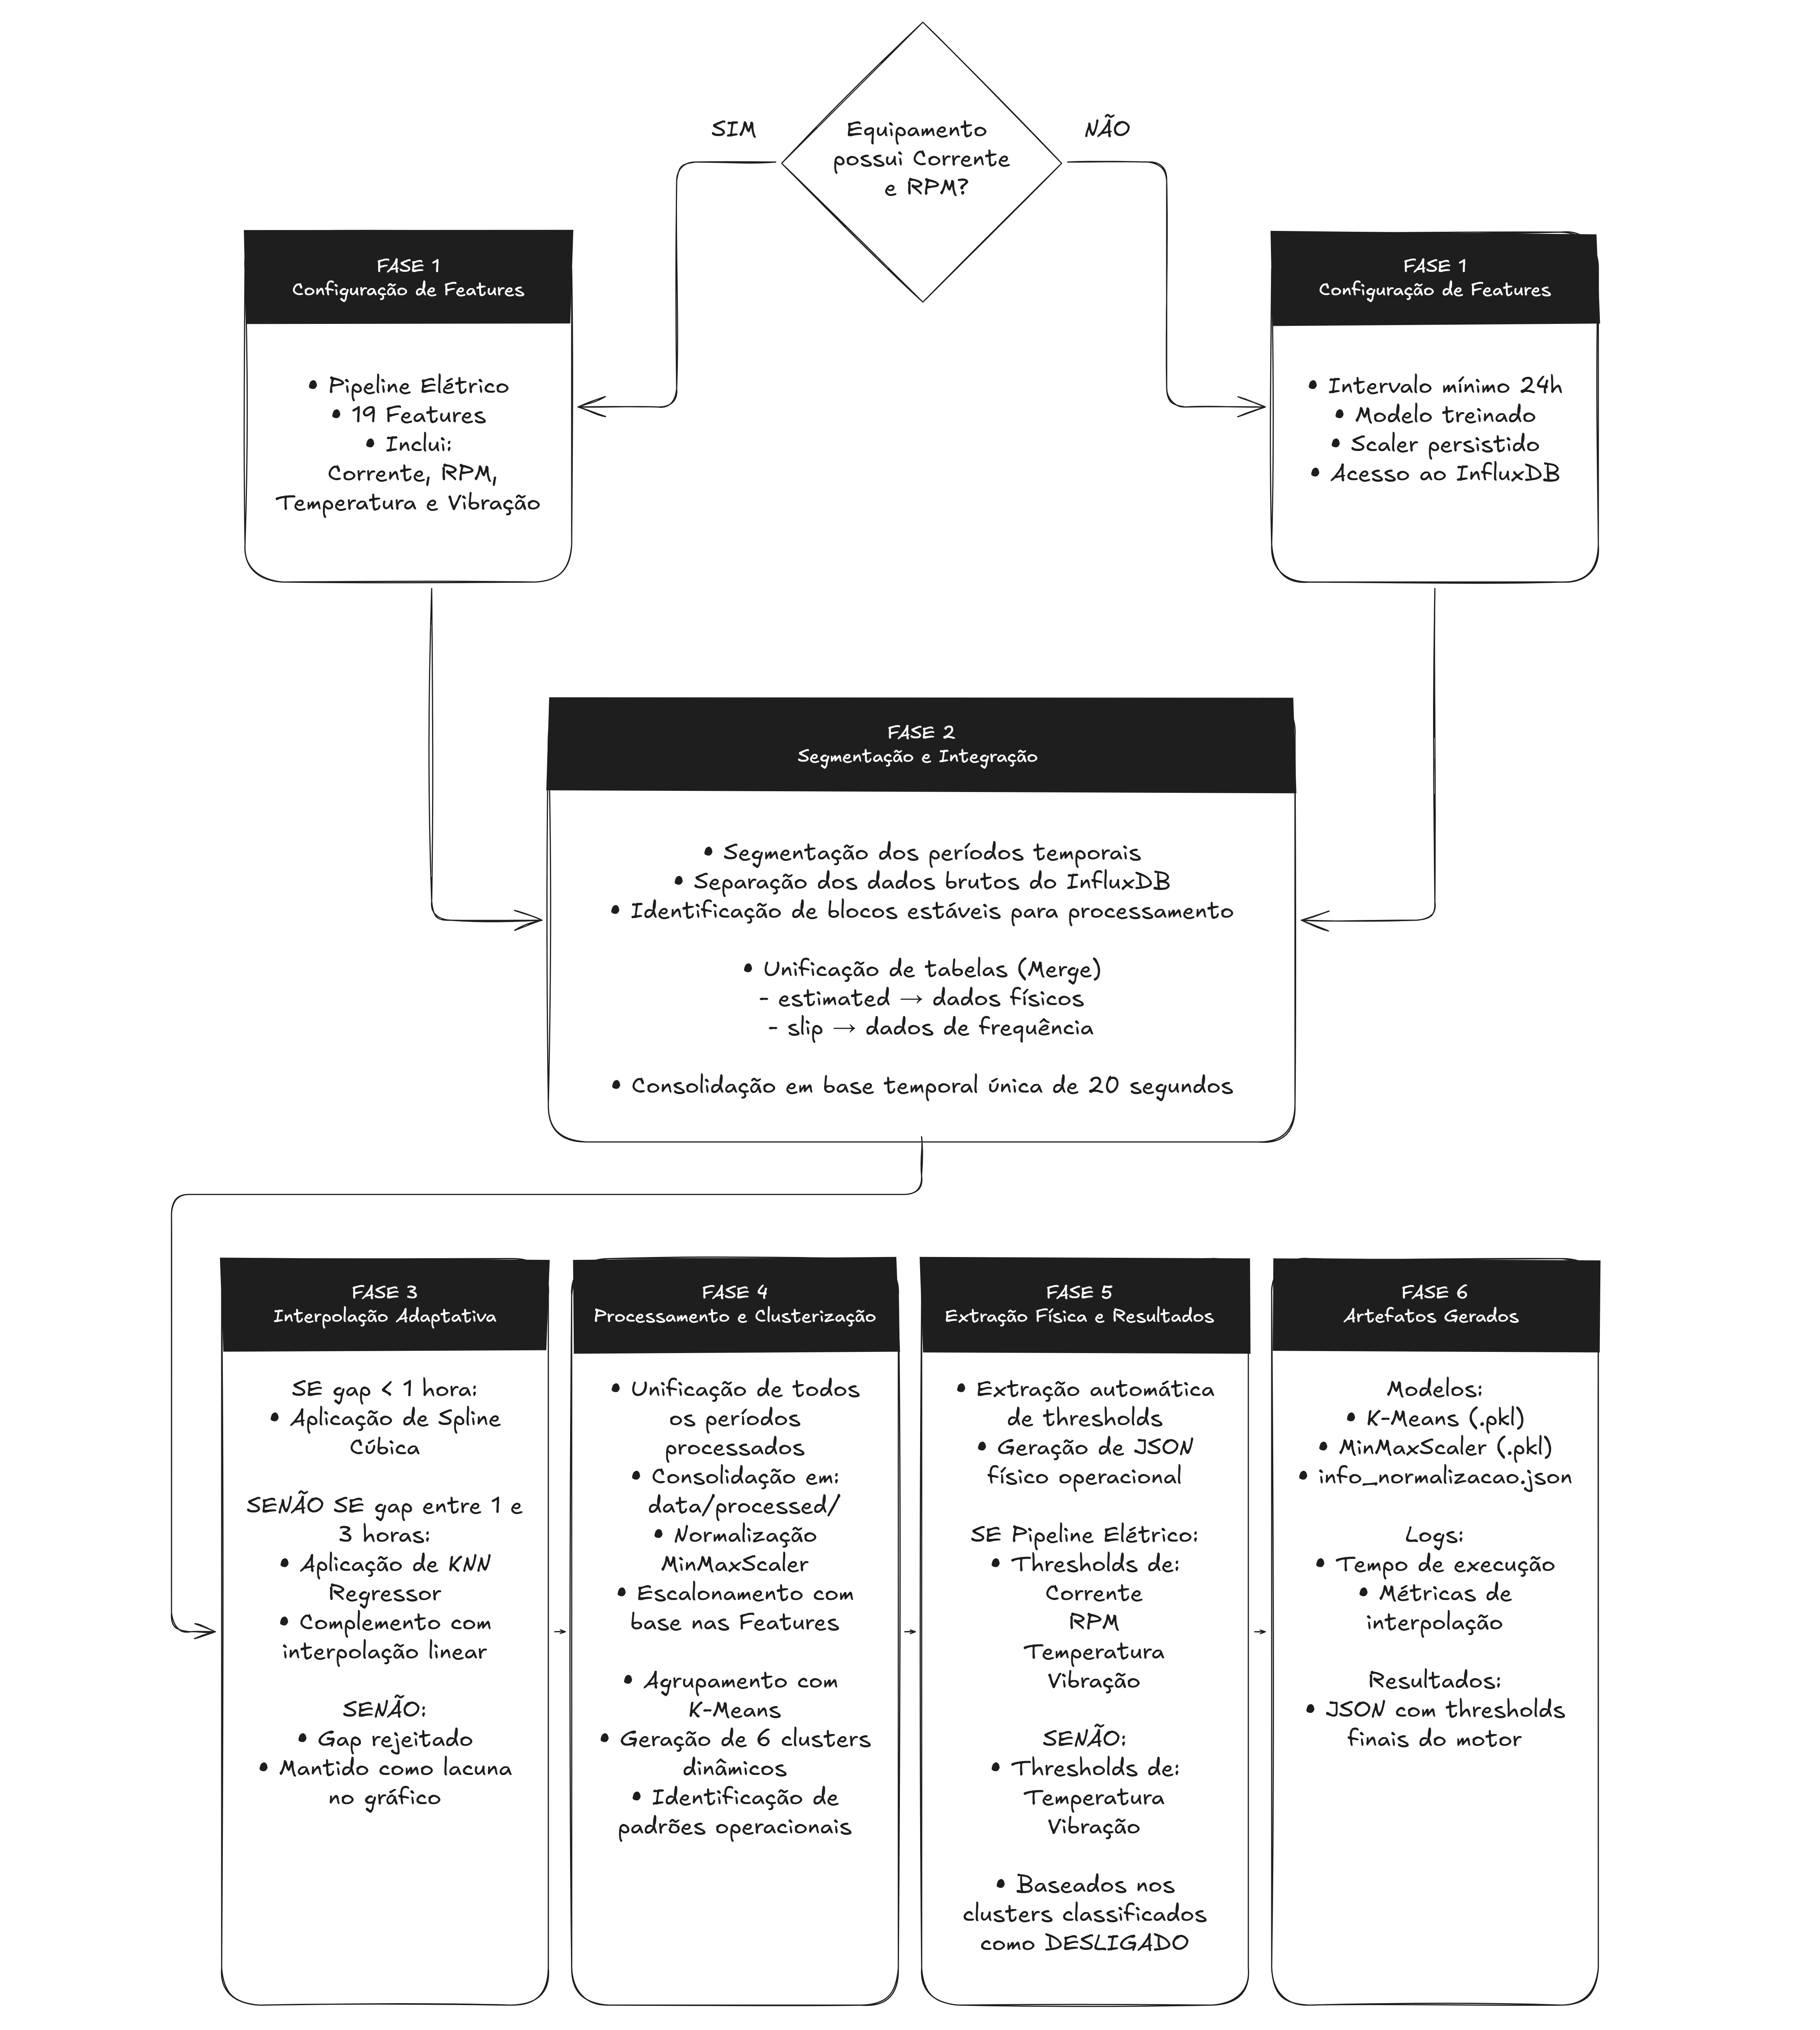
\includegraphics[width=0.5\textwidth]{plots/05_pipeline_treino.png}
    \caption{Fluxo de treinamento unificado para os modelos K-Means (Elétrico e Mecânico). O diagrama ilustra as seis fases do processo: (1) Configuração condicional de \textit{features}; (2) Segmentação e unificação de dados; (3) Preenchimento adaptativo de lacunas via Spline Cúbica ou KNN; (4) Clusterização K-Means; (5) Extração automática de limites operacionais (\textit{thresholds}); e (6) Geração dos artefatos persistentes (.pkl e .json).}
    \label{fig:pipeline_treino}
\end{figure}

\section{Coleta de Dados e Processamento}

O sistema adapta automaticamente a coleta de dados baseada no tipo de equipamento identificado. Equipamentos elétricos utilizam três fontes: \texttt{validated\_default} (frequência de amostragem de 20 segundos) com magnitude magnética em 3 eixos, temperatura do objeto e velocidade máxima/RMS em 3 eixos; \texttt{estimated} (frequência de amostragem de aproximadamente 1 minuto) com velocidade rotacional (RPM), vibração RMS estimada e corrente elétrica em amperes; e \texttt{validated\_slip} (frequência de amostragem de 2 minutos) com frequência de escorregamento, magnitudes e RMS. Equipamentos mecânicos utilizam apenas duas fontes: \texttt{validated\_default} e \texttt{validated\_slip}, sem dados de corrente e RPM.

O sistema implementa uma estratégia otimizada de \textit{download} que verifica a existência de arquivos locais completos para cada equipamento. Se existe, carrega localmente e filtra em Python para evitar \textit{timeouts} no InfluxDB. Caso contrário, baixa o intervalo específico via consulta SQL. Esta estratégia foi necessária devido a \textit{timeouts} em consultas grandes (acima de 1 milhão de registros). O sistema aceita entrada em GMT-3 (horário de Brasília) e converte automaticamente para UTC antes de consultar o InfluxDB, adicionando 3 horas ao horário fornecido.

\section{Segmentação e Validação}

O processamento inicia com a segmentação temporal dos dados. Para equipamentos elétricos, o sistema carrega arquivos CSV brutos com marcações temporais e sensores, converte marcações temporais para formato \textit{datetime} (UTC), ordena dados cronologicamente e valida presença de colunas obrigatórias: \texttt{time}, \texttt{mag\_x}, \texttt{mag\_y}, \texttt{mag\_z}, \texttt{object\_temp}, \texttt{vel\_max\_x/y/z}, \texttt{vel\_rms\_x/y/z} e \texttt{m\_point} para a fonte \texttt{validated\_default}; \texttt{rotational\_speed}, \texttt{current} e \texttt{vel\_rms} para \texttt{estimated}; e \texttt{fe\_frequency}, \texttt{fe\_magnitude}, \texttt{fr\_frequency} e \texttt{rms} para \texttt{validated\_slip}. O sistema calcula diferenças temporais entre amostras consecutivas e identifica quebras de continuidade quando a diferença é maior que 3 horas, atribuindo ID único a cada período contínuo e registrando metadados.

Cada período deve atender critérios de validação: duração mínima de 24 horas, presença de dados obrigatórios (rotational\_speed, current, vel\_rms e dados de \textit{slip} para elétricos; temperature e vel\_rms para mecânicos) e continuidade temporal sem lacunas excessivas. Para períodos válidos, gera-se uma linha temporal uniforme com marcações de 20 em 20 segundos. Equipamentos mecânicos seguem processo similar, mas focam em sensores de temperatura e vibração, sem exigir dados de RPM e corrente.

\section{Processamento e Interpolação}

O sistema executa detecção de \textit{outliers} por IQR (\textit{Interquartile Range})~\cite{tukey1977iqr} aplicado a cada coluna/sensor individualmente. Utiliza multiplicador conservador 3,0 (\textit{versus} 1,5 tradicional) para calcular limites inferior e superior, marcando valores \textit{outliers} como NaN. Adicionalmente, foi implementada uma trava de segurança dinâmica contra alucinações de sensores causadas por Interferência Eletromagnética (EMI). Como os sensores magnéticos calculam RPM e corrente lendo a distorção do campo magnético, ruídos de fontes externas (como o acionamento de motores vizinhos ou proximidade de cabos de alta tensão) podem levar o magnetômetro a captar campos espúrios. Nestes casos, o sensor pode registrar erroneamente altas rotações (ex: $> 100$ RPM) acompanhadas de correntes nulas ou irrisórias, mesmo com o eixo físico da máquina parado e vibração absoluta nula. Para neutralizar esse artefato sem distorcer os dados, o código calcula o Percentil 90 (P90) da corrente válida de cada motor. O P90 é uma medida estatística que indica o valor abaixo do qual se encontram 90\% das amostras; neste contexto, ele é utilizado como um estimador robusto do nível de corrente de operação nominal, sendo menos sensível a picos isolados de partida ou ruídos transitórios do que a média aritmética simples. Se o RPM indicar operação, mas a corrente não acompanhar (permanecendo abaixo de 5\% do P90 ou menor que $2,0$ A), o sistema classifica o pico como uma "falsa partida" por interferência e zera forçadamente tanto o RPM quanto a corrente. Isso impede que os picos fantasmas propaguem classificações errôneas de LIGADO no algoritmo K-Means.

A Figura~\ref{fig:limpeza_outliers_iqr} ilustra o processo completo de detecção e limpeza automática de uma motobomba elétrica de $125~\text{cv}$. No gráfico superior, observam-se picos de vibração RMS na faixa de 30 a 60 mm/s, valores fisicamente impossíveis para uma motobomba industrial em operação normal. Segundo a norma ISO 10816-3~\cite{iso10816_3}, equipamentos industriais dessa classe operam tipicamente com vibração RMS abaixo de 7,1 mm/s (Zona C -- alerta), sendo que valores acima desse limiar já indicam condição crítica. Picos da ordem de 60 mm/s são, portanto, inequivocamente artefatos espúrios causados por interferências eletromagnéticas ou falhas momentâneas do sensor, e não representam condição operacional real do equipamento. Após a limpeza automática pelo IQR, o gráfico inferior mostra o sinal tratado e contínuo, com valores coerentes dentro da faixa operacional esperada.

\begin{figure}[H]
    \centering
    
\includegraphics[width=0.75\textwidth]{plots/04_remocao_outliers.png}
    \caption{Processo de detecção e limpeza automática de \textit{outliers} utilizando o método IQR (\textit{Interquartile Range}). Superior: Sinal bruto com picos anômalos (\textit{outliers} físicos) superiores a 30 mm/s, valores fisicamente impossíveis segundo a ISO 10816-3~\cite{iso10816_3}, detectados acima do limiar calculado. Inferior: Sinal tratado e contínuo após a remoção automática.}
    \label{fig:limpeza_outliers_iqr}
\end{figure}

Como a operação industrial respeita a lei da inércia, sequências de $\geq 10$ amostras consecutivas identificadas como \textit{outlier} são preservadas, o que garante a proteção de sequências operacionais e evita a remoção de estados de desligamento legítimos (ex: RPM=0 ou vibração nula), que poderiam ser estatisticamente classificados como \textit{outliers} em períodos de longa operação. Esta abordagem preserva variações operacionais legítimas. Para cada período válido, gera-se uma linha temporal completa com marcações de 20 em 20 segundos.

A interpolação adaptativa emprega três estratégias baseadas no tamanho da lacuna. A escolha da técnica de interpolação é motivada pelas características específicas de cada método e pelo nível de confiabilidade exigido para diferentes tamanhos de lacuna, considerando o \textit{trade-off} entre robustez da estimativa e custo computacional.

Para lacunas de até 30 minutos (90 amostras a 20 segundos), utiliza-se o interpolador PCHIP (\textit{Piecewise Cubic Hermite Interpolating Polynomial})~\cite{fritsch1980pchip}. Diferentemente da \textit{spline} cúbica padrão, o PCHIP garante monotonicidade local entre os pontos de dados, o que significa que a curva interpolada segue a tendência dos dados sem criar oscilações artificiais. Inicialmente, testou-se a \textit{spline} cúbica convencional, que apresentou oscilações espúrias (\textit{overshoot}) em lacunas maiores --- um comportamento associado ao fenômeno de Runge~\cite{runge1901phenomenon}, no qual a interpolação por polinômios de grau elevado em pontos equidistantes pode gerar oscilações crescentes nas extremidades do intervalo, produzindo valores fisicamente impossíveis. O PCHIP evita esse problema ao ajustar as derivadas nos pontos de junção para preservar a forma local dos dados. Também foi avaliada a utilização de redes LSTM (\textit{Long Short-Term Memory})~\cite{hochreiter1997lstm} para reconstrução de lacunas, porém a complexidade computacional superior não resultou em ganho de qualidade frente ao KNN, conforme ilustrado na Figura~\ref{fig:comparativo_knn_lstm}. A Figura~\ref{fig:interpolacao_spline_exemplo} ilustra o comportamento do PCHIP em uma lacuna real. Nota-se que a curva interpolada (em laranja) apresenta transição suave e contínua entre os dados originais (em azul), sem descontinuidades ou oscilações artificiais, preservando a tendência natural do sinal.

\begin{figure}[H]
    \centering
    
\includegraphics[width=0.85\textwidth]{plots/02_spline_interpolacao.png}
    \caption{Exemplo de interpolação temporal de lacuna utilizando o interpolador PCHIP (\textit{Piecewise Cubic Hermite Interpolating Polynomial}). A curva interpolada (laranja) reconstrói o sinal de vibração RMS com transição suave, contínua e monótona, preservando a tendência natural dos dados originais (azul) sem oscilações artificiais~\cite{fritsch1980pchip}.}
    \label{fig:interpolacao_spline_exemplo}
\end{figure}

\newpage

Do ponto de vista computacional, a interpolação PCHIP possui complexidade $O(n)$ para $n$ pontos de dados~\cite{fritsch1980pchip}, sendo extremamente eficiente. O KNN temporal, por sua vez, possui complexidade $O(n \cdot k)$ onde $k$ é o número de vizinhos~\cite{cover1967nearest, bishop2006pattern}, representando custo moderado. O K-Means utilizado na classificação possui complexidade $O(n \cdot k \cdot d \cdot i)$, onde $n$ é o número de amostras, $k$ o número de \textit{clusters}, $d$ a dimensionalidade e $i$ o número de iterações~\cite{arthur2007k, bishop2006pattern}, tornando-o viável mesmo para milhões de registros.

Para lacunas entre 30 minutos e 3 horas, utiliza-se uma combinação de K-Nearest Neighbors (KNN) temporal (peso 0,6) com interpolação linear (peso 0,4). O KNN temporal busca os $k$ pontos mais próximos no eixo temporal e estima o valor faltante com base na média ponderada desses vizinhos, capturando padrões cíclicos e tendências locais que a interpolação linear sozinha não conseguiria representar. A interpolação linear, por sua vez, fornece uma estimativa conservadora e monotônica que evita oscilações. A combinação ponderada dos dois métodos equilibra a capacidade do KNN de capturar padrões complexos com a estabilidade da interpolação linear. A Figura~\ref{fig:interpolacao_knn_exemplo} demonstra o resultado desta abordagem combinada em uma lacuna real.

\begin{figure}[H]
    \centering
    
\includegraphics[width=0.85\textwidth]{plots/02_knn_interpolacao.png}
    \caption{Exemplo de interpolação temporal de lacuna utilizando o algoritmo KNN. O gráfico demonstra a recomposição suave do sinal de vibração RMS no intervalo onde houve perda de dados originais, com dados originais (antes e depois da lacuna) em azul e valores interpolados (KNN) em azul claro.}
    \label{fig:interpolacao_knn_exemplo}
\end{figure}

Para lacunas maiores que 3 horas, optou-se por não interpolar, criando período separado. Esta decisão é justificada pelo fato de que, em intervalos tão longos, o estado do equipamento pode ter mudado completamente (por exemplo, de LIGADO para DESLIGADO), e qualquer tentativa de interpolação introduziria viés significativo nos dados, comprometendo a confiabilidade da classificação posterior.

Equipamentos mecânicos seguem lógica similar mas focam em temperatura como sensor principal e análise de vibração para estados operacionais, sem processar dados de RPM e corrente.

Cada valor interpolado recebe indicador de qualidade: 1,00 para dados originais, 0,95 para interpolação PCHIP e 0,75 para interpolação KNN. Esta marcação permite rastrear a confiabilidade ao longo do \textit{pipeline}.

\section{Junção e Sincronização}

O sistema combina dados de múltiplas fontes em linha temporal unificada. Para equipamentos elétricos, utiliza \texttt{validated\_\allowbreak default} (20 s) como linha temporal base, \texttt{estimated} (aproximadamente 1 minuto) para RPM e corrente, e \texttt{validated\_\allowbreak slip} (2 minutos) para análise de frequência. O processo identifica períodos correspondentes com sobreposição temporal maior que 70\%, realiza junção temporal por alinhamento de marcações temporais e sincronização multifrequência usando preenchimento retroativo (\textit{backward-fill}): tolerância de 6 minutos para \texttt{estimated} e 3 minutos para \texttt{validated\_\allowbreak slip}, evitando preenchimento prospectivo (\textit{forward-fill}) que poderia usar dados futuros. O \textit{backward-fill}~\cite{mckinney2010pandas} é uma técnica de preenchimento de dados faltantes que propaga o próximo valor válido para trás no tempo, ou seja, um dado ausente recebe o valor da próxima leitura futura mais próxima. Inversamente, o \textit{forward-fill} propaga o último valor válido para frente. A escolha pelo \textit{backward-fill} neste contexto é conservadora: garante que a sincronização utilize apenas dados que já existem na linha temporal, sem extrapolar valores passados para janelas futuras.

Equipamentos mecânicos utilizam apenas \texttt{validated\_\allowbreak default} e \texttt{validated\_\allowbreak slip}, focando na sincronização entre temperatura/vibração e análise de frequência. O sistema aplica os seguintes critérios de validação a cada período: (i) ausência de lacunas consecutivas maiores que 3 horas, caso contrário o período é segmentado; (ii) presença de todos os sensores necessários (\texttt{object\_temp}, \texttt{vel\_rms\_x/y/z}, \texttt{mag\_x/y/z} para \texttt{validated\_\allowbreak default}; \texttt{fe\_\allowbreak frequency}, \texttt{rms} para \texttt{validated\_\allowbreak slip}); (iii) consistência temporal, verificando que as marcações temporais são estritamente monotônicas (crescentes); e (iv) sobreposição mínima adequada entre as fontes \texttt{validated\_\allowbreak default} e \texttt{validated\_\allowbreak slip}, garantindo que exista um intervalo temporal compartilhado suficiente para a junção. Períodos que não atendem a esses critérios são automaticamente descartados com registro detalhado em \textit{log}, incluindo o motivo da rejeição e as estatísticas do período.

\section{Normalização}

O sistema normaliza os dados preparando-os para clusterização. Para equipamentos elétricos, normaliza 19 atributos incluindo magnetômetro (mag\_x/y/z), temperatura (object\_temp), picos e RMS de vibração (vel\_max e vel\_rms em 3 eixos), RPM (rotational\_speed), corrente elétrica (current) e dados de \textit{slip} (fe\_frequency, fe\_magnitude, fr\_frequency, rms). Para equipamentos mecânicos, normaliza 16 atributos focados em magnetômetro, temperatura como sensor principal, picos e RMS de vibração em 3 eixos e dados de \textit{slip}.

O processo aplica normalização MinMax~\cite{minmax_sklearn}, escalando para intervalo $[0,1]$, tratando \textit{outliers} com \textit{clipping} no percentil 99,5\% e preservando a distribuição relativa dos dados. A Figura~\ref{fig:minmax_scaler} comprova que a normalização MinMax não altera a distribuição estatística dos dados: a forma, a dispersão e os padrões dos sinais originais são integralmente preservados após a transformação, sendo modificada apenas a escala dos valores. Conforme documentado por Pedregosa et al.~\cite{minmax_sklearn}, o MinMaxScaler aplica uma transformação linear $X_{\text{norm}} = \frac{X - X_{\min}}{X_{\max} - X_{\min}}$, que por ser estritamente monotônica, preserva a ordem relativa e a distribuição dos dados originais.

\begin{figure}[H]
    \centering
    
\includegraphics[width=0.85\textwidth]{plots/01_minmax_scaler.png}
    \caption{Comparação entre dados brutos (esquerda) e dados normalizados (direita) pelo MinMax. A normalização preserva integralmente a distribuição estatística dos sinais, alterando apenas a escala para o intervalo $[0,1]$, sem distorcer a forma nem a dispersão dos dados originais~\cite{minmax_sklearn}.}
    \label{fig:minmax_scaler}
\end{figure}

O MinMaxScaler treinado é persistido para garantir normalização consistente de novos dados, reprodutibilidade de resultados e aplicação em produção sem re-treinamento.

\section{Classificação K-Means Adaptativa}

O algoritmo K-Means é configurado com $k=6$ \textit{clusters}, inicialização \textit{k-means++} inteligente, 10 inicializações, máximo de 300 iterações e \textit{random state} 42 para reprodutibilidade. A escolha de $k=6$ permite capturar diferentes regimes operacionais: estados puramente desligado, estados de \textit{standby}/transição e estados de operação em diferentes cargas/intensidades.

A Figura~\ref{fig:kmeans_animacao} ilustra a convergência do algoritmo K-Means ao longo das iterações. Utilizou-se $k=6$ \textit{clusters}, e os centróides convergem para posições que representam os diferentes regimes operacionais. Na escala de cores, tons de verde mais escuros indicam valores mais elevados dos atributos (maior atividade operacional), enquanto tons de vermelho mais escuros representam valores mais baixos (menor atividade ou equipamento desligado). A animação completa está disponível no repositório do projeto (\href{https://1drv.ms/i/c/5f1c3aa3f12af1a2/IQBjyXW5EjddQaIrD6MY6jblAR4XaUFGNN3yKheuEY8MA7E?e=CTUrx6}{\texttt{03\_kmeans\_animacao.gif}}), pois o formato GIF não é suportado com animação em documentos PDF.

\begin{figure}[H]
    \centering
    
\includegraphics[width=0.75\textwidth]{plots/03_kmeans_animacao.png}
    \caption[Convergência do algoritmo K-Means com $k=6$ \textit{clusters}]{Convergência do algoritmo K-Means com $k=6$ \textit{clusters}. Os centróides (marcadores em destaque) convergem para posições representativas de cada regime operacional. Verde escuro: valores elevados dos atributos; vermelho escuro: valores baixos. Animação completa disponível em: \href{https://1drv.ms/i/c/5f1c3aa3f12af1a2/IQBjyXW5EjddQaIrD6MY6jblAR4XaUFGNN3yKheuEY8MA7E?e=CTUrx6}{\texttt{03\_kmeans\_animacao.gif}}.}
    \label{fig:kmeans_animacao}
\end{figure}

Após a clusterização, os \textit{clusters} são classificados automaticamente em LIGADO ou DESLIGADO baseado em \textit{scores} ponderados. Para equipamentos elétricos, o \textit{score} é calculado pela fórmula:

\begin{equation}
    S_{eletrico} = 2{,}0 \cdot \bar{C}_{corrente} + 2{,}0 \cdot \bar{C}_{RPM} + 1{,}0 \cdot \bar{C}_{vibracao} + 0{,}5 \cdot \bar{C}_{temperatura}
    \label{eq:score_eletrico}
\end{equation}

\noindent onde $\bar{C}_{x}$ representa a média normalizada do atributo $x$ no centróide do \textit{cluster}, priorizando corrente e RPM como sinais mais confiáveis. Para equipamentos mecânicos, o \textit{score} é dado por:

\begin{equation}
    S_{mecanico} = 1{,}5 \cdot \bar{C}_{temperatura} + 1{,}0 \cdot \bar{C}_{vibracao} + 0{,}5 \cdot \bar{C}_{magnetometro}
    \label{eq:score_mecanico}
\end{equation}

Os \textit{clusters} são ordenados por \textit{score} crescente com preferência conservadora: 1 \textit{cluster} com menor \textit{score} é classificado como DESLIGADO, e os 5 restantes como LIGADO. Entretanto, \textit{clusters} adicionais podem ser incluídos na categoria DESLIGADO se atenderem a critérios rigorosos de similaridade: (i) diferença de \textit{score} inferior a 0,3 em relação ao primeiro cluster, com \textit{score} absoluto abaixo de 0,5; e (ii) vibração máxima do cluster candidato não exceder em mais de 30\% a vibração máxima do \textit{cluster} base (limiar de vibração residual). Um exemplo típico ocorre quando o equipamento possui dois estados de repouso distintos (ex: motor parado com ventilação desligada vs. motor parado com vibração residual de máquinas adjacentes), onde ambos apresentam sinais elétricos nulos e vibrações mínimas.

Adicionalmente, implementou-se uma trava de segurança denominada \textit{Vibration Safety Floor}: independente do \textit{score} ou da ausência de dados elétricos, qualquer \textit{cluster} com vibração normalizada acima de um limiar fixo de segurança (0,06 para elétricos e 0,08 para mecânicos) é obrigatoriamente classificado como LIGADO. Esta proteção garante que o sistema identifique corretamente a operação mesmo em estados de baixa carga ou quando sensores de corrente/RPM falham, evitando que estados operacionais ruidosos sejam erroneamente classificados como repouso devido a falhas de instrumentação elétrica.

O sistema calcula e persiste limiares específicos para cada equipamento baseado no percentil 95\% dos dados do \textit{cluster} DESLIGADO, salvos como valores físicos reais (não normalizados) para comparação direta com valores reais em análises futuras. O modelo K-Means treinado é persistido junto com metadados incluindo atributos utilizados, classificação dos \textit{clusters}, estatísticas e data de treinamento.

\section{Análise por Intervalo e Validação}

O sistema implementa análise por intervalo com validações rigorosas exigindo cobertura temporal maior que 70\% e lacunas consecutivas menores que 10 minutos. Valores 0,0 são válidos e representam equipamento desligado; o que invalida são lacunas temporais (ausência de dados). A lógica de máxima rigorosidade ordena \textit{clusters} por \textit{score} crescente, classificando apenas o \textit{cluster} de menor \textit{score} como DESLIGADO inicialmente, incluindo um segundo \textit{cluster} apenas se atender critérios rigorosos, garantindo que apenas estados inequivocamente desligados sejam classificados como tal.

Na análise de intervalos, a classificação usa limiares reais específicos do equipamento salvos durante o treinamento, comparando valores físicos reais sem necessidade de uma nova normalização. O equipamento é classificado como DESLIGADO se corrente, RPM e vibração estiverem todos abaixo dos limiares calculados, ou se corrente e RPM estiverem baixos com vibração residual até 3,0 mm/s. Cada equipamento usa seus próprios limiares calculados dinamicamente, priorizando corrente e RPM como sinais mais confiáveis.

O sistema implementa filtros de limpeza de dados incluindo filtro de \textit{outliers} temporais que corrige classificações espúrias (sequências menores que 10 minutos), filtro de \textit{outliers} por IQR~\cite{tukey1977iqr} removendo valores fisicamente impossíveis, filtro de continuidade temporal validando lacunas menores que 3 horas, validação de atributos obrigatórios garantindo presença de sensores críticos e verificação de consistência temporal. Equipamentos elétricos validam simultaneamente RPM, corrente e vibração, enquanto mecânicos validam temperatura \textit{versus} vibração.

Este \textit{pipeline} de análise por intervalo, acessível através da aba de Análise de Intervalo do sistema (Figura~\ref{fig:gui_intervalo}), é utilizado para classificar novos períodos de dados após a conclusão do treinamento do modelo. O processo opera em cinco fases, conforme ilustrado na Figura~\ref{fig:pipeline_cinco_fases}: validação de requisitos (intervalo mínimo 24 horas, modelo treinado, \textit{scaler} persistido e acesso ao InfluxDB), extração e validação (conversão GMT-3 para UTC, \textit{download} de dados e validação de cobertura temporal maior que 70\%), processamento (segmentação temporal, interpolação adaptativa e sincronização multifrequência), classificação avançada (predição K-Means, correção por limiares físicos e filtro de \textit{outliers} temporais) e análise de métricas calculando tempo em cada estado considerando durações temporais reais.

\begin{figure}[H]
    \centering
    
\includegraphics[width=0.95\textwidth]{plots/05_pipeline_cinco_fases.png}
    \caption{Visão geral das cinco fases do \textit{pipeline} completo de análise por intervalo. Cada fase é executada sequencialmente: a validação de requisitos garante a existência de modelos e dados; a extração obtém e valida os dados brutos; o processamento aplica segmentação, interpolação e sincronização; a classificação avançada utiliza K-Means com correção por limiares físicos; e a análise de métricas calcula os tempos efetivos em cada estado operacional.}
    \label{fig:pipeline_cinco_fases}
\end{figure}

O sistema oferece interface interativa com entrada de datas em formato brasileiro, tratamento robusto de erros com \textit{retry} e \textit{backoff} exponencial, \textit{cache} inteligente evitando re-\textit{download} desnecessário, \textit{logs} estruturados com rastreabilidade completa e visualizações automáticas com gráficos 3D e relatórios detalhados. Para equipamentos mecânicos, algoritmo especial seleciona intervalos 3D otimizando balanceamento de tempo ligado/desligado, número de transições e qualidade dos dados.

\section{Implementação}

O sistema foi implementado em Python 3.11 utilizando arquitetura modular com \textit{scripts} especializados para equipamentos elétricos e mecânicos. Equipamentos elétricos utilizam 8 \textit{scripts} principais cobrindo \textit{download} de 3 fontes de dados (\texttt{validated\_\allowbreak default} a 20 s, \texttt{estimated} a aproximadamente 1 minuto e \texttt{validated\_\allowbreak slip} a 2 minutos), segmentação com interpolação KNN temporal, processamento detalhado por período, junção multifrequência com sincronização, normalização MinMax de 19 atributos e treinamento K-Means com visualizações. Equipamentos mecânicos utilizam 7 \textit{scripts} adaptados processando apenas 2 fontes de dados (\texttt{validated\_\allowbreak default} e \texttt{validated\_\allowbreak slip}), focando em temperatura e vibração, e normalizando 16 atributos específicos.

O sistema utiliza \textit{pandas}~\cite{mckinney2010pandas} para manipulação de dados temporais, \textit{scikit-learn} para K-Means e normalização, \textit{scipy} para interpolação PCHIP e KNN, \textit{matplotlib} para visualizações 3D e InfluxDB para conexão com banco de dados. Para processar 1 milhão de registros são necessários 8--16 GB de RAM, 5--10 minutos de processamento e 500 MB a 2 GB de armazenamento para dados e modelos.

\subsection{Estrutura de Diretórios do Projeto}

A organização do código-fonte, dados, modelos e resultados segue uma estrutura hierárquica e padronizada, onde o sufixo \texttt{c\_\{\{m\_mpoint\}\}} representa dinamicamente o identificador único de cada equipamento industrial (ex: \texttt{c\_636} que é um equipamento elétrico e \texttt{c\_1518}, que é mecânico):

\begin{verbatim}
/
|-- GUI.bat                                # Atalho para execucao
|-- README.md                              # Documentacao do projeto
|-- desktop.ini                            # Configuracao de pasta
|-- code/                                  # Diretorio de codigo-fonte
|   |-- gui_pipeline.py   # Interface grafica unificada
|   |-- pipeline_deteccao_estados.py    # Orquestrador ELETRICO
|   |-- pipeline_deteccao_estados_mecanico.py # Orquestrador MECANICO
|-- data/
|   |-- raw/   # Dados brutos do InfluxDB
|   |   |-- dados_c_{{m_mpoint}}.csv
|   |   |-- dados_slip_c_{{m_mpoint}}.csv
|   |   +-- dados_estimated_c_{{m_mpoint}}.csv
|   |-- raw_preenchido/   # Dados processados e interpolados
|   |   |-- periodo_{XX}_c_{{m_mpoint}}.csv
|   |   |-- periodo_{XX}_slip_c_{{m_mpoint}}.csv
|   |   |-- periodo_{XX}_estimated_c_{{m_mpoint}}.csv
|   |   +-- periodo_{XX}_final_c_{{m_mpoint}}.csv
|   |-- processed/   # Dados unificados e classificados
|   |   |-- dados_unificados_final_c_{{m_mpoint}}.csv
|   |   +-- dados_classificados_kmeans_moderado_c_{{m_mpoint}}.csv
|   +-- normalized/   # Dados prontos para ML
|       +-- dados_kmeans_c_{{m_mpoint}}.csv
|-- models/
|   +-- c_{{m_mpoint}}/   # Modelos e configuracoes
|       |-- config_c_{{m_mpoint}}.json
|       |-- kmeans_model_moderado_c_{{m_mpoint}}.pkl
|       |-- scaler_model_moderado_c_{{m_mpoint}}.pkl
|       |-- info_kmeans_model_moderado_c_{{m_mpoint}}.json
|       +-- info_normalizacao_c_{{m_mpoint}}.json
|-- results/
|   +-- c_{{m_mpoint}}/   # Visualizacoes e Relatorios
|       |-- analise_kmeans_clusters_moderado_c_{{m_mpoint}}.png
|       |-- analise_kmeans_clusters_mecanico_c_{{m_mpoint}}.png
|       |-- dados_normalizados_analise_c_{{m_mpoint}}_mecanico.png
|       |-- vibracao_reconstrucao_c_{{m_mpoint}}.png
|       |-- estados_temperatura_vibracao_tempo_3d_1_c_{{m_mpoint}}.png
|       |-- relatorio_treinamento_c_{{m_mpoint}}_mecanico.txt
|       +-- results_c_{{m_mpoint}}.txt
|-- logs/   # Logs de execucao por etapa
|   |-- pipeline_deteccao_estados_complete_c_{{m_mpoint}}_{ts}.txt
|   |-- kmeans_classificacao_moderado_complete_c_{{m_mpoint}}_{ts}.txt
|   +-- normalizar_dados_kmeans_complete_c_{{m_mpoint}}_{ts}.txt
|-- scripts/                               # Modulos de processamento
|   |-- baixar_*.py                        # Scripts de coleta
|   |-- processar_dados_simples*.py        # Limpeza e interpolacao
|   |-- unir_sincronizar_periodos*.py      # Uniao de sensores
|   |-- normalizar_dados_kmeans*.py        # Preparo para K-means
|   |-- kmeans_classificacao*.py           # Treino e classificacao
|   |-- analise_intervalo_completa*.py     # Injecao e analise
|   +-- plot_vibracao_temporal_colorido.py # Visualizacao avancada
+-- utils/                                 # Utilitarios de suporte
    |-- artifact_paths.py                  # Gestor de caminhos
    |-- logging_utils.py                   # Gestor de logs
    +-- lista_mpoints.txt                  # Cadastro de hardwares
\end{verbatim}

\section{Interface Gráfica do Sistema}

O sistema implementa uma interface gráfica intuitiva desenvolvida em Python usando a biblioteca Tkinter, facilitando a operação do \textit{pipeline} completo sem necessidade de conhecimento técnico em programação. A interface está organizada em três abas principais, cada uma responsável por uma etapa específica do processo.

\subsection{Aba de Treinamento}

A primeira aba (Figura~\ref{fig:gui_treino}) permite o treinamento de modelos K-Means para múltiplos equipamentos. O sistema detecta automaticamente quais equipamentos possuem dados disponíveis e identifica seu tipo (ELÉTRICO ou MECÂNICO).

\begin{figure}[H]
    \centering
    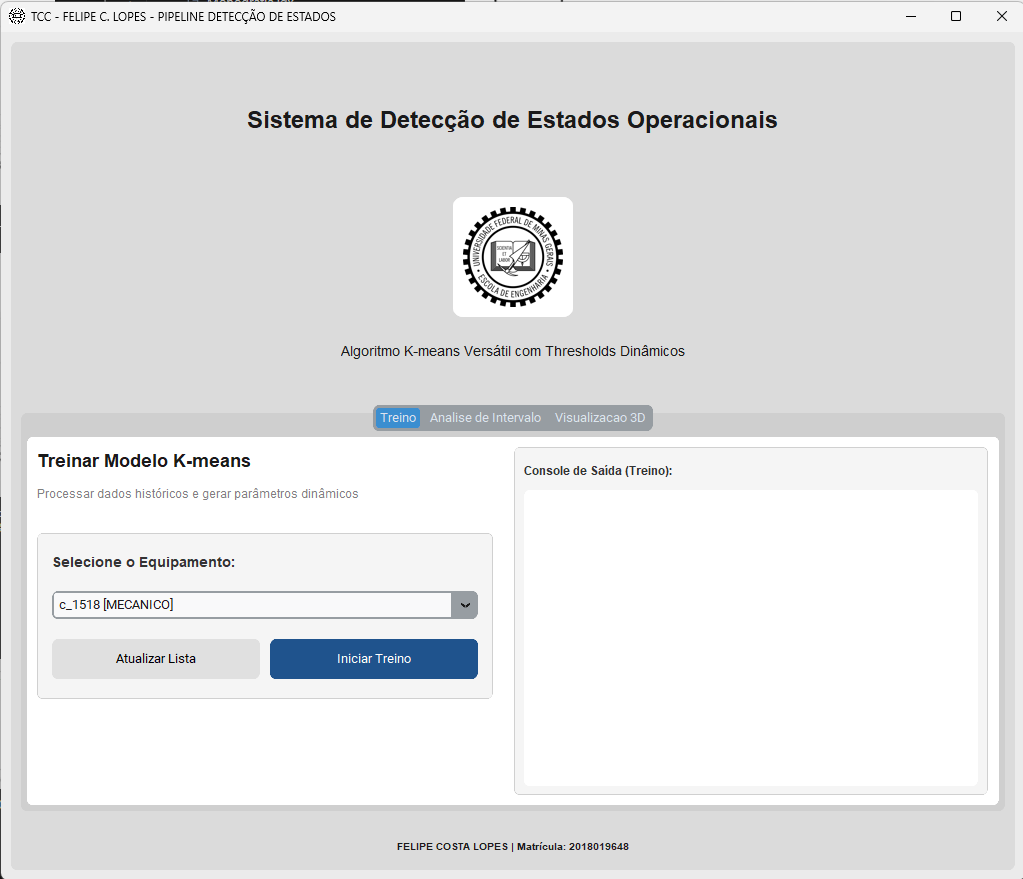
\includegraphics[width=0.5\textwidth]{results/gui_treino.png}
    \caption{Interface gráfica -- Aba de Treinamento.}
    \label{fig:gui_treino}
\end{figure}

Funcionalidades da Aba de Treinamento: O sistema identifica equipamentos com dados disponíveis, distingue automaticamente entre equipamentos elétricos e mecânicos, exibe \textit{logs} em tempo real do processo de treinamento através de console de saída, oferece botão para recarregar equipamentos disponíveis e executa \textit{pipeline} completo para todos os equipamentos listados.

\subsection{Aba de Análise por Intervalo}

A segunda aba (Figura~\ref{fig:gui_intervalo}) permite análise de períodos específicos consultando dados diretamente do InfluxDB em tempo real, ideal para investigação de anomalias ou validação de períodos customizados.

\begin{figure}[H]
    \centering
    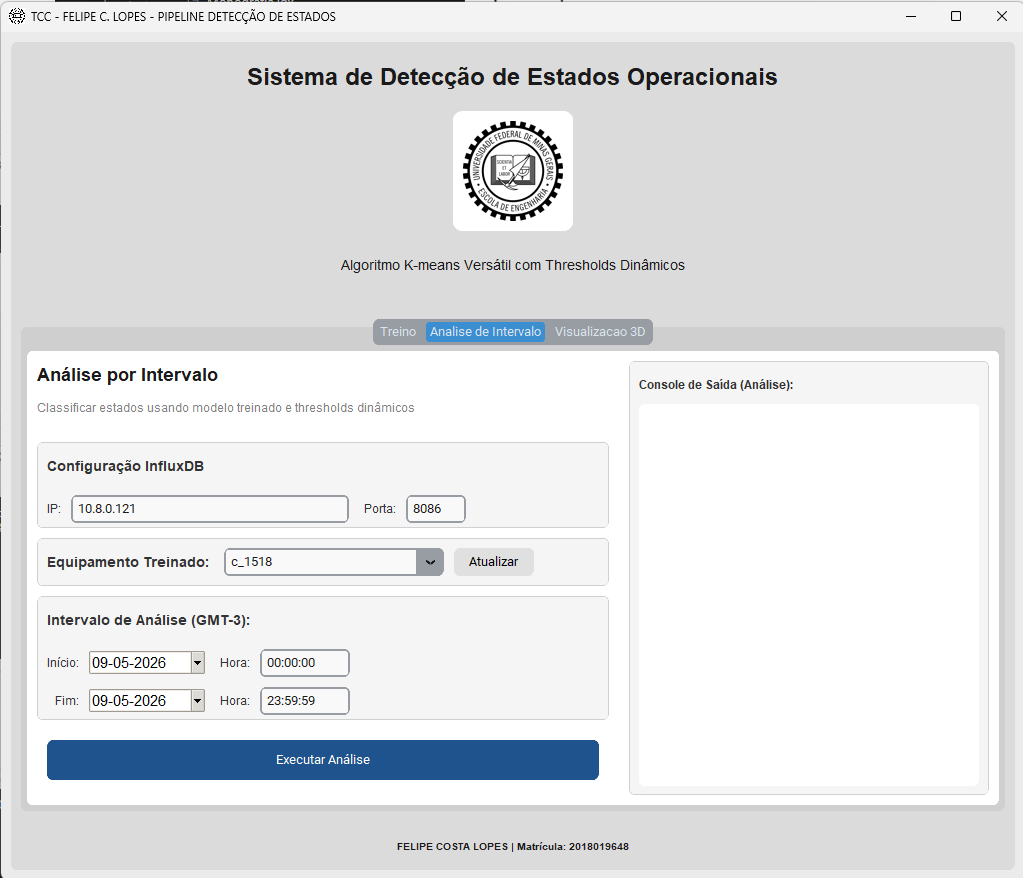
\includegraphics[width=0.5\textwidth]{results/gui_intervalo.png}
    \caption{Interface gráfica -- Aba de Análise por Intervalo. Configuração de conexão InfluxDB (IP e porta), seleção de equipamento, definição de intervalo temporal (GMT-3) e execução de análise customizada.}
    \label{fig:gui_intervalo}
\end{figure}

Funcionalidades da Aba de Análise por Intervalo: Permite configuração do InfluxDB com IP (10.8.0.XXX) e porta (8086) configuráveis, seleção de equipamento através de \textit{dropdown} com todos os equipamentos treinados, definição de intervalo temporal com seletores de data/hora para início e fim (GMT-3), recarga da lista de equipamentos com modelos disponíveis, execução de análise que baixa dados do período, aplica modelo treinado e classifica estados, e console de saída mostrando progresso de \textit{download}, processamento e resultados.

\newpage

\subsection{Aba de Visualização 3D}

A terceira aba (Figura~\ref{fig:gui_visualizacao}) gera visualizações tridimensionais dos \textit{clusters} K-Means e estados operacionais classificados, permitindo inspeção visual da qualidade da clusterização.

\begin{figure}[H]
    \centering
    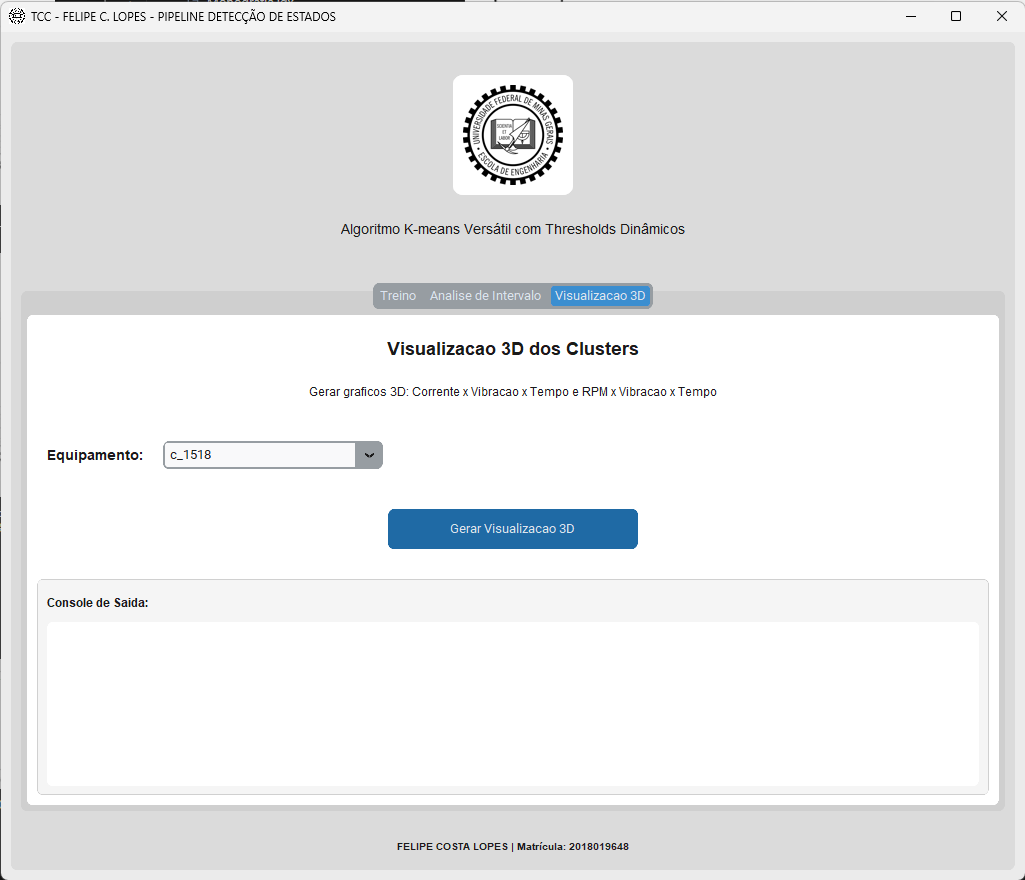
\includegraphics[width=0.5\textwidth]{results/gui_visualizacao.png}
    \caption{Interface gráfica -- Aba de Visualização 3D. Seleção de equipamento e geração automática de gráficos 3D: Corrente $\times$ Vibração $\times$ Tempo e RPM $\times$ Vibração $\times$ Tempo (equipamentos elétricos) ou Temperatura $\times$ Vibração $\times$ Tempo (equipamentos mecânicos).}
    \label{fig:gui_visualizacao}
\end{figure}

Funcionalidades da Aba de Visualização 3D: Permite seleção entre equipamentos com modelos treinados, cria automaticamente gráficos tridimensionais, adapta gráficos por tipo de equipamento (RPM para elétricos, Temperatura para mecânicos), aplica coloração por estado (verde para LIGADO, vermelho para DESLIGADO) e salva automaticamente gráficos no diretório results/.

\subsection{Arquitetura da Interface}

A interface gráfica está implementada no arquivo \texttt{gui\_pipeline.py} seguindo princípios de separação de responsabilidades onde cada aba encapsula uma funcionalidade específica do \textit{pipeline}, \textit{feedback} em tempo real com console de saída atualizado durante execução das tarefas, validações automáticas do sistema antes de processar, tratamento de erros com mensagens claras em caso de falhas e execução assíncrona que não bloqueia a interface durante operações longas.

\clearpage